\documentclass[a4paper,12pt,notitlepage]{article}
\usepackage{fullpage}
%\setkomafont{disposition}{\normalfont\bfseries}
%\usepackage{setspace}
%\setstretch{1.5}
\usepackage{graphicx}
\usepackage{tikz}
\usetikzlibrary{shapes,arrows,positioning}
\usepackage[style=authoryear,backend=biber]{biblatex}
\renewcommand*{\nameyeardelim}{\addcomma\addspace}
\usepackage[toc,page]{appendix}
\usepackage{textcomp}
\usepackage{amsmath}
\usepackage{mathtools}
\usepackage{listings}
\usepackage{color}
\usepackage{hyperref}
\addbibresource{report.bib}
\graphicspath{{res/images/}}

\begin{document}

\parskip 2mm

\title{{\huge Playing Card Recognition}\\\vspace{2 mm}{\large \textbf{Computer Vision (EE4H) --- Final Report}}}
%\subtitle{EECE MEng4 FYP -– Second Report}
\author{Yousef Amar (1095307)\\Chris Lewis (1234567)}
\date{2014-04-28}
\maketitle
\thispagestyle{empty}
\vfill
%\begin{quotation}
\begin{abstract}
	Lorem ipsum dolor sit amet, consectetur adipisicing elit, sed do eiusmod tempor incididunt ut labore et dolore magna aliqua. Ut enim ad minim veniam, quis nostrud exercitation ullamco laboris nisi ut aliquip ex ea commodo consequat. Duis aute irure dolor in reprehenderit in voluptate velit esse cillum dolore eu fugiat nulla pariatur. Excepteur sint occaecat cupidatat non proident, sunt in culpa qui officia deserunt mollit anim id est laborum.
\end{abstract}
%\end{quotation}
\pagebreak

%\addtocontents{toc}{\protect\thispagestyle{empty}}
\tableofcontents
\thispagestyle{empty}
\pagebreak
\setcounter{page}{1}

\parskip 2mm

\section{Introduction}
	
	This is a paragraph. Here's an example of cross-referencing: please see Review (section \ref{sec:review} on page \pageref{sec:review}).

	\subsection{Project Specification}

		This is a \emph{subsection}. Whitespace is mostly meaningless in \LaTeX. Indenting with tabs is just useful for collapsing parts of the document you aren't working on in Sublime; it has no effect on document appearance. Speaking of Sublime, these are some useful packages for working in \LaTeX:

		\begin{enumerate}
			\item ``LaTeXTools'' (better than ``LaTeXing'') because
			\begin{enumerate}
				\item Doesn't pester you to buy it
				\item Has pretty good syntax highlighting and auto completion
				\item Auto completion for cross-referencing figures/sections/appendices and citations too
				\item Includes LaTeX build system --- Ctrl+B to compile; no command line headaches
			\end{enumerate}
			\item Edit your settings file for really smooth spell check: \url{http://www.sublimetext.com/docs/3/spell_checking.html}
			\item ``Origami'' for multiple panes in Sublime --- useful to have notes open as a clipboard on the side
			\item ``Increment Selection'' (came in handy once or twice)
		\end{enumerate}

\pagebreak

\section{Review}
\label{sec:review}

	Here's another section. Here's a figure with 0.8 of the line width:

	\begin{figure}[ht]
		\centering
		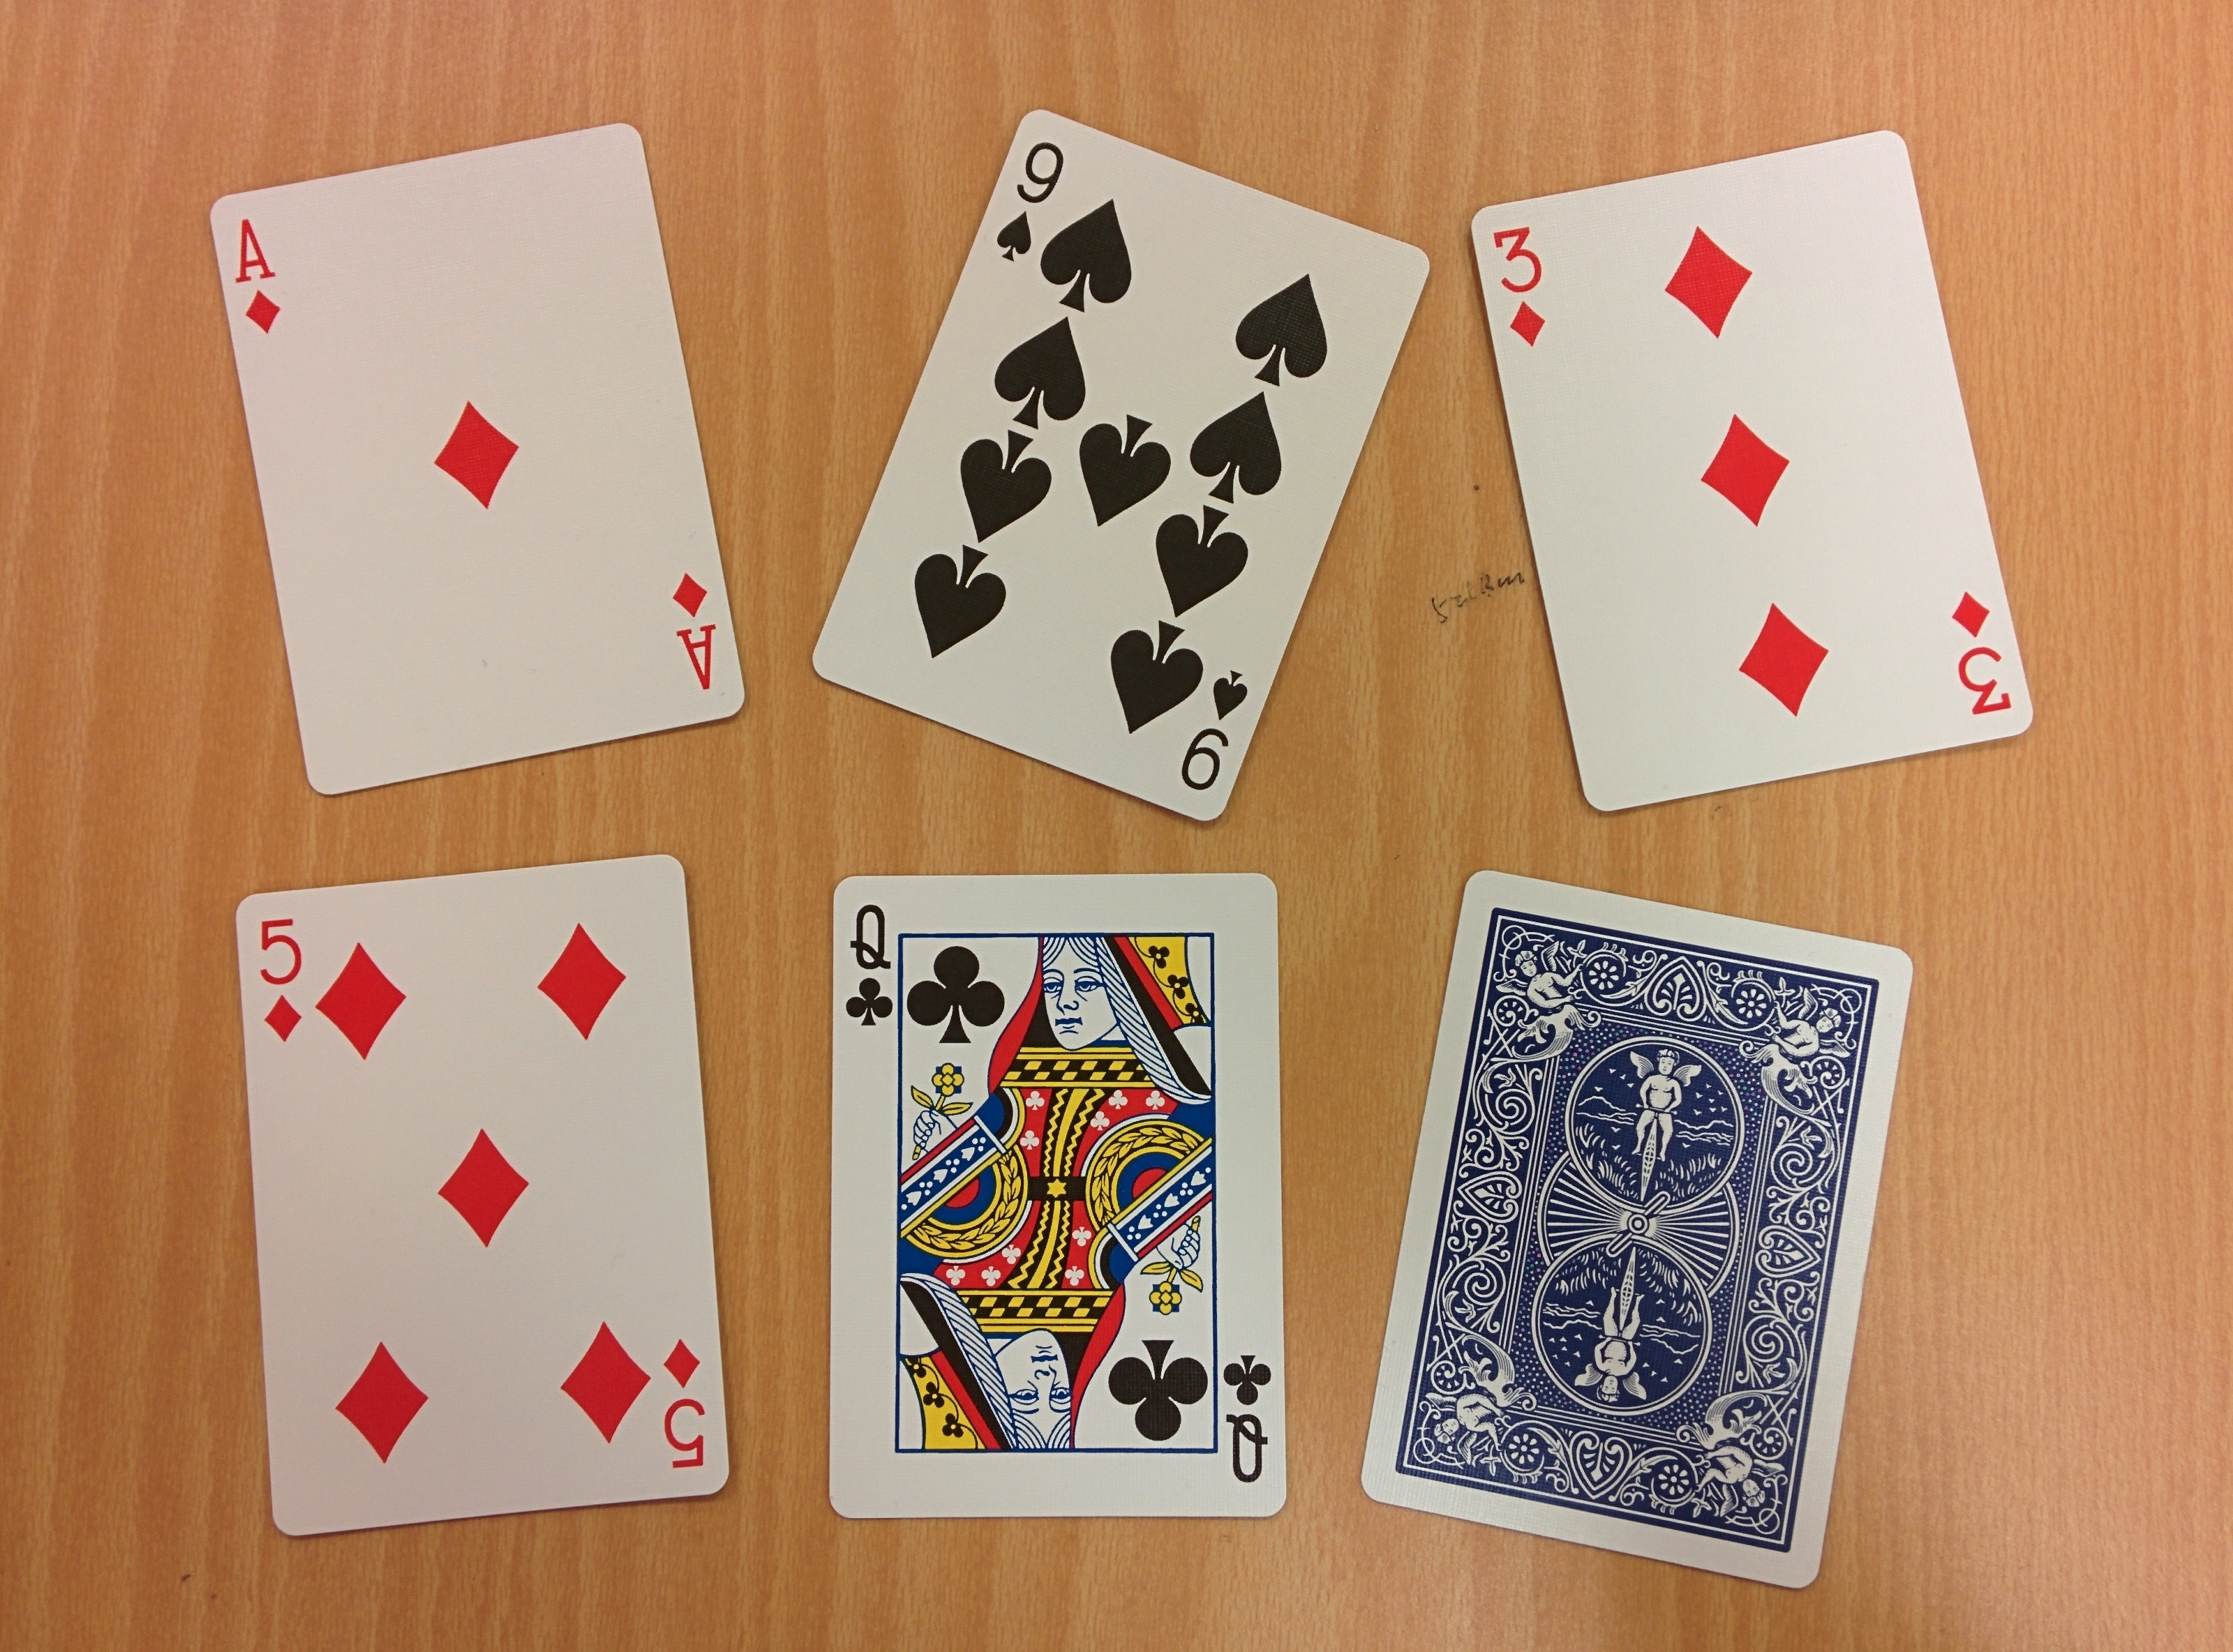
\includegraphics[width=0.8\linewidth]{mixed}
		\caption{Example of Card}
		\label{fig:mixed}
	\end{figure}

	\LaTeX is pretty good at figuring out what to do with figure. There are a number of options for them too that are cool. Here's me cross-referencing the figure without breaking a sweat: please see figure \ref{fig:mixed} on page \pageref{fig:mixed}.

\pagebreak

\section{Proposed Method}

	\LaTeX is really good at equations. Here's a simple one from my report:

	$$x = \frac{ct}{2} - \epsilon$$

	Want some confusion matrices? Here are some matrix examples from my final report:

	\begin{equation*}
		T =
		\begin{bmatrix}
			84 & 200 & 16 \\
			56 & 238 & 11 \\
			251 & 206 & 203
		\end{bmatrix}
		\qquad
		I =
		\begin{bmatrix}
			160 & 40 & 250 & 27 & 114 \\
			81 & 94 & 14 & 100 & 37 \\
			225 & 52 & 148 & 137 & 111
		\end{bmatrix}
	\end{equation*}

	Here's me sprinkling some math inline: $\theta$, $x$ and $y$, $I_1$ and $I_2$, $|T - I_n|$. Want some graphs? Google pgfplots and prepare to be blown away.

\pagebreak

\section{Implementation}
	
	You can also put a lot of stuff in one figure even on different lines:
	
	\begin{figure}[ht]
		\centering
		
\includegraphics[width=0.2\linewidth]{cards/jackofclubs}
		
\includegraphics[width=0.2\linewidth]{cards/kingofdiamonds}
		
\includegraphics[width=0.2\linewidth]{cards/queenofhearts}\\[5px]
		
\includegraphics[width=0.3\linewidth]{cards/2ofdiamonds}
		
\includegraphics[width=0.3\linewidth]{cards/3ofclubs}
		\caption{Example of Cards}
		\label{fig:stuff}
	\end{figure}

\pagebreak

\section{Evaluation}
	
	See appendix \ref{app:maincpp} on page \pageref{app:maincpp} for an example of code listings. The style is completely customisable of course. Notice also that it's not copied to the \emph{appendices} directory, it's just a symlink to \emph{src}! According to this random book off of Google Scholar, computer vision is pretty cool \autocite{forsyth2002computer}. I use BibLatex + Biber to compile the bibliography; the order is ``latexmk'' (or build), ``biber report'', then ``latexmk'' again. This only needs to be done if the bibliography changes and then it might as well be done only really at the very end when the report is finished to so don't worry about it. LaTeXing does it automatically but it's not worth it.

\pagebreak

\section{Conclusion}

	We've only just scratched the surface! Here, have a mini flow chart:

	% Define block styles
	\tikzstyle{decision} = [diamond, draw, fill=blue!20, text badly centered, inner sep=0pt, text width=4em, font=\tiny]
	\tikzstyle{process} = [rectangle, draw, fill=blue!20, text centered, rounded corners, text width=3em, font=\tiny]
	\tikzstyle{line} = [draw, -latex', font=\tiny]
	\tikzstyle{cloud} = [draw, ellipse, fill=red!20, minimum height=2em]
	
	\begin{figure}[ht]
		\centering
		\begin{tikzpicture}[node distance = 2cm, auto]
			% Place nodes
			\node [process] (imgget) {Get Image from File/Webcam};
			\node [process, right of=imgget] (cardfind) {Isolate Cards};
			\node [process, right of=cardfind] (colourdet) {Detect Colour};
			\node [process, right of=colourdet] (typedet) {Detect Type};
			\node [process, right of=typedet] (symfind) {Isolate Symbols};
			\node [decision, right of=symfind] (ispic) {Is Card Picture Type?};
			\node [process, above right of=ispic] (numdet) {Detect Number};
			\node [process, below right of=ispic] (rankdet) {Detect Rank};
			% Enhanced by colour detection
			\node [process, below right of=numdet] (symdet) {Detect Suit};


			% Draw edges
			\path [line] (imgget) -- (cardfind);
			\path [line] (cardfind) -- (colourdet);
			\path [line] (colourdet) -- (typedet);
			\path [line] (typedet) -- (symfind);
			\path [line] (symfind) -- (ispic);
			\path [line] (ispic) -- node {no} (numdet);
			\path [line] (ispic) -- node [below left] {yes} (rankdet);
			\path [line] (rankdet) -- (symdet);
			\path [line] (numdet) -- (symdet);
			%\path [line,dashed] (expert) -- (init);
			%\path [line,dashed] (system) -- (init);
			%\path [line,dashed] (system) |- (evaluate);
		\end{tikzpicture}
		\caption{Top-level Flowchart}
		\label{fig:flowchart}
	\end{figure}

\pagebreak

\thispagestyle{empty}
\printbibliography

\pagebreak

\begin{appendices}

\definecolor{bluekeywords}{rgb}{0.13,0.13,1}
\definecolor{greencomments}{rgb}{0,0.5,0}
\definecolor{redstrings}{rgb}{0.9,0.7,1}

\section{Source Code Listings}

% Here's where you can mess with the style (this is a comment btw)
\lstset{
	language=C++,
	showspaces=false,
	showtabs=false,
	breaklines=true,
	breakatwhitespace=true,
	escapeinside={(*@}{@*)},
	commentstyle=\color{greencomments},
	keywordstyle=\color{bluekeywords},
	stringstyle=\color{redstrings},
	basicstyle=\ttfamily\scriptsize,
	captionpos=t,
	extendedchars=true,
	frame=single,
	keepspaces=true,
	showstringspaces=false,
	stepnumber=2,
	tabsize=2,
}

\subsection{main.cpp}
\label{app:maincpp}
\lstinputlisting{res/appendices/src/main.cpp}

\end{appendices}

\vfill
\hrulefill

\end{document}